\documentclass[tikz,border=10pt]{standalone}
\usetikzlibrary{calc}
\begin{document}
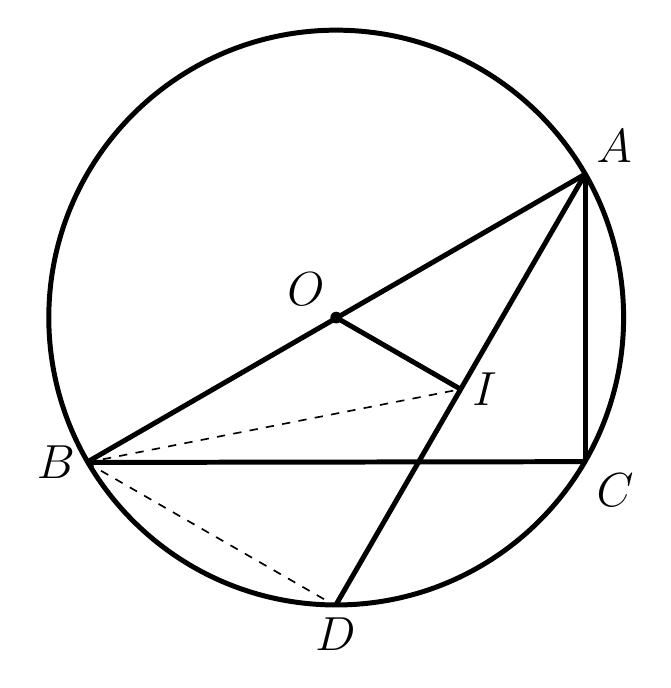
\begin{tikzpicture}[line join=round, line width=1.8pt]
% Coordinates: s = 0.015474 units/px, y flipped about py=268
\coordinate (A) at (3.17,2.17);
\coordinate (B) at (-3.16,-1.49);
\coordinate (C) at (3.17,-1.48);
\coordinate (D) at (0.00,-3.31);
\coordinate (O) at (0.01,0.35);
\coordinate (I) at (1.59,-0.56);
\coordinate (P) at (1.05,-1.49);

% Circle (full, thick)
\draw (O) circle (3.65);

% Solid segments
\draw (A) -- (B);   % diameter through O
\draw (A) -- (C);
\draw (B) -- (C);
\draw (A) -- (D);   % through I and P
\draw (O) -- (I);

% Dashed segments: thin, standard dashed pattern (unchanged)
\draw[dashed, draw=black, line width=0.6pt] (B) -- (I);
\draw[dashed, draw=black, line width=0.6pt] (B) -- (D);

% Labels
\node[font=\fontsize{18}{21.6}\selectfont, above right] at (A) {$A$};
\node[font=\fontsize{18}{21.6}\selectfont, left] at (B) {$B$};
\node[font=\fontsize{18}{21.6}\selectfont, below right] at (C) {$C$};
\node[font=\fontsize{18}{21.6}\selectfont, below] at (D) {$D$};
\node[font=\fontsize{18}{21.6}\selectfont, above left] at (O) {$O$};
\node[font=\fontsize{18}{21.6}\selectfont, right] at (I) {$I$};

% Centre dot at O: explicit node, drawn last so nothing covers it
\node[circle, fill=black, inner sep=1.5pt] at (O) {};
\end{tikzpicture}
\end{document}